\fancyhead[L]{\textbf{68}\quad \textbf{\textsf{CHƯƠNG 1}}\quad Các hàm số và Mô hình}
\fancyhead[R]{}

\noindent
{\color{stewartcyan}\Huge\textbf{\textsf{BÀI TẬP}}}\\[-0.5em]
{\color{stewartcyan}\rule{\textwidth}{1.5pt}}\bigskip

\noindent
\begin{minipage}[t]{0.485\textwidth}
\begin{enumerate}[label=\textbf{\arabic*.}, leftmargin=*]
    \item Cho $f$ là hàm số có đồ thị như hình bên dưới.
    \begin{center}
        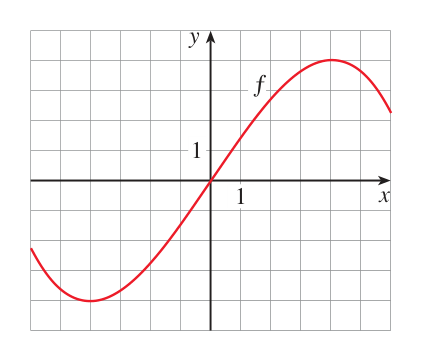
\includegraphics[width=0.62\linewidth]{images/p0103_fig1.png}
    \end{center}
    \begin{enumerate}[label=(\alph*), itemsep=1pt]
        \item Ước lượng giá trị của $f(2)$.
        \item Ước lượng các giá trị của $x$ sao cho $f(x) = 3$.
        \item Tìm tập xác định của $f$.
        \item Tìm tập giá trị của $f$.
        \item Hàm số $f$ đồng biến trên khoảng nào?
        \item $f$ có phải là hàm đơn ánh không? Giải thích.
        \item $f$ là hàm chẵn, lẻ hay không chẵn cũng không lẻ? Giải thích.
    \end{enumerate}

    \item Cho đồ thị của hàm số $g$.
    \begin{center}
        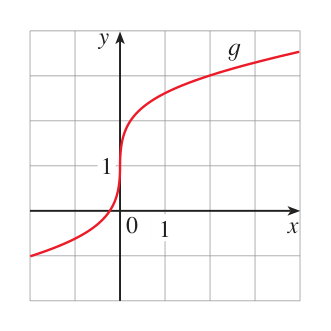
\includegraphics[width=0.55\linewidth]{images/p0103_fig2.png}
    \end{center}
    \begin{enumerate}[label=(\alph*), itemsep=1pt]
        \item Xác định giá trị của $g(2)$.
        \item Vì sao $g$ là hàm đơn ánh?
        \item Ước lượng giá trị của $g^{-1}(2)$.
        \item Ước lượng tập xác định của $g^{-1}$.
        \item Vẽ phác thảo đồ thị của $g^{-1}$.
    \end{enumerate}

    \item Cho hàm số $f(x) = x^2 - 2x + 3$, hãy tính tỉ số gia (tỉ sai phân)
    \[
    \frac{f(a+h) - f(a)}{h}
    \]

    \item Hãy vẽ phác thảo đồ thị năng suất cây trồng như là một hàm số theo lượng phân bón sử dụng.
\end{enumerate}

\noindent
{\color{stewartcyan}\textbf{5--8}}\; Tìm tập xác định và tập giá trị của mỗi hàm số sau. Viết kết quả dưới dạng ký hiệu khoảng.
\begin{multicols}{2}
\begin{enumerate}[label=\textbf{\arabic*.}, leftmargin=*, resume]
    \item $f(x) = 2/(3x - 1)$
    \item $g(x) = \sqrt{16 - x^4}$
    \item $h(x) = \ln(x + 6)$
    \item $F(t) = 3 + \cos 2t$
\end{enumerate}
\end{multicols}

\begin{enumerate}[label=\textbf{\arabic*.}, leftmargin=*, resume]
    \item Giả sử đã cho đồ thị của $f$. Hãy mô tả cách để thu được đồ thị của các hàm số sau từ đồ thị của $f$.
    \begin{multicols}{2}
    \begin{enumerate}[label=(\alph*), itemsep=1pt]
        \item $y = f(x) + 5$
        \item $y = f(x + 5)$
        \item $y = 1 + 2f(x)$
        \item $y = f(x - 2) - 2$
        \item $y = -f(x)$
        \item $y = f^{-1}(x)$
    \end{enumerate}
    \end{multicols}
\end{enumerate}
\end{minipage}%
\hfill
\begin{minipage}[t]{0.485\textwidth}
\begin{enumerate}[label=\textbf{\arabic*.}, leftmargin=*, resume]
    \item Cho đồ thị của $f$. Hãy vẽ đồ thị của các hàm số sau.
    \begin{multicols}{2}
    \begin{enumerate}[label=(\alph*), itemsep=1pt]
        \item $y = f(x - 8)$
        \item $y = -f(x)$
        \item $y = 2 - f(x)$
        \item $y = \frac{1}{2}f(x) - 1$
        \item $y = f^{-1}(x)$
        \item $y = f^{-1}(x + 3)$
    \end{enumerate}
    \end{multicols}
    \begin{center}
        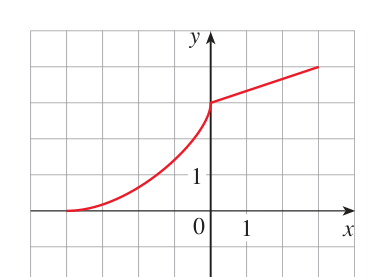
\includegraphics[width=0.62\linewidth]{images/p0103_fig3.png}
    \end{center}
\end{enumerate}

\noindent
{\color{stewartcyan}\textbf{11--18}}\; Sử dụng các phép biến đổi đồ thị để phác thảo đồ thị của mỗi hàm số.
\begin{multicols}{2}
\begin{enumerate}[label=\textbf{\arabic*.}, leftmargin=*, resume]
    \item $f(x) = x^3 + 2$
    \item $f(x) = (x - 3)^2$
    \item $y = \sqrt{x + 2}$
    \item $y = \ln(x + 5)$
    \item $g(x) = 1 + \cos 2x$
    \item $h(x) = -e^x + 2$
    \item $s(x) = 1 + 0.5^x$
    \item $f(x) = \begin{cases} -x & \text{nếu } x < 0 \\ e^x - 1 & \text{nếu } x \ge 0 \end{cases}$
\end{enumerate}
\end{multicols}

\begin{enumerate}[label=\textbf{\arabic*.}, leftmargin=*, resume]
    \item Xác định xem hàm số $f$ là chẵn, lẻ hay không chẵn cũng không lẻ.
    \begin{multicols}{2}
    \begin{enumerate}[label=(\alph*), itemsep=1pt]
        \item $f(x) = 2x^5 - 3x^2 + 2$
        \item $f(x) = x^3 - x^7$
        \item $f(x) = e^{-x^2}$
        \item $f(x) = 1 + \sin x$
        \item $f(x) = 1 - \cos 2x$
        \item $f(x) = (x + 1)^2$
    \end{enumerate}
    \end{multicols}

    \item Tìm công thức xác định hàm số có đồ thị gồm đoạn thẳng nối từ điểm $(-2, 2)$ đến điểm $(-1, 0)$ kết hợp với nửa trên của đường tròn tâm tại gốc tọa độ và bán kính bằng $1$.

    \item Cho $f(x) = \ln x$ và $g(x) = x^2 - 9$, hãy tìm các hàm số hợp: (a) $f \circ g$, (b) $g \circ f$, (c) $f \circ f$, (d) $g \circ g$, và tìm tập xác định của chúng.

    \item Hãy biểu diễn hàm số $F(x) = 1/\sqrt{x + \sqrt{x}}$ dưới dạng hợp tử của ba hàm số.

    \item Tuổi thọ trung bình đã được cải thiện rõ rệt trong những thập kỷ gần đây. Bảng sau cung cấp tuổi thọ kỳ vọng khi sinh (tính theo năm) của nam giới tại Hoa Kỳ. Hãy sử dụng biểu đồ phân tán để chọn loại mô hình thích hợp. Sử dụng mô hình của bạn để dự đoán tuổi thọ của một bé trai sinh vào năm 2030.

    \begin{center}
    \small
    \begin{tabular}{|c|c||c|c|}
        \hline
        \rowcolor{stewartcyan!20}
        \textbf{Năm sinh} & \textbf{Tuổi thọ} & \textbf{Năm sinh} & \textbf{Tuổi thọ} \\
        \hline
        1900 & 48.3 & 1960 & 66.6 \\
        1910 & 51.1 & 1970 & 67.1 \\
        1920 & 55.2 & 1980 & 70.0 \\
        1930 & 57.4 & 1990 & 71.8 \\
        1940 & 62.5 & 2000 & 73.0 \\
        1950 & 65.6 & 2010 & 76.2 \\
        \hline
    \end{tabular}
    \end{center}
\end{enumerate}
\end{minipage}